Since the wave equation is time reversible, it suffices to consider the problem in one direction of time. To unify the notation, we consider the global well-posedness problem starting at time $t = 1$ backwards-in-time and the scattering problem starting at time $t = 0$ forwards-in-time. Assume towards a contradiction that the theorem fails, e.g. $\phi$ is a solution on $t \in (0, 1]$ blowing up as $t \downarrow 0$ or a global solution on $t \in[0, \infty)$ which fails to scatter $||\phi||_{\sfS[0, \infty)} = +\infty$. We claim that, after translating and rescaling, it suffices to consider solution which are regular outside of the forward light cone $C$, e.g.
	\begin{equation}\tag{$\epsilon_*$}\label{eq:exterior}
		\cE_{(\{t\} \times \R^3) \setminus S_t} [\phi[t]] \leq \epsilon_*.
	\end{equation}
This follows from the small data theory, smooth localisation of the energy, finite speed of propagation, and energy-flux decay. 

\subsection{Non-scattering scenario}

Suppose towards a contradiction that given finite energy data at time $t = 0$ the solution is global yet fails to scatter as $t \to \infty$. We localise by remarking that the energy-flux identity implies the energy exterior to a large light cone remains small for all time, and so the solution can be regarded as regular in view of small data theory. Indeed, by monotone convergence we can find a large ball $B_{R_*} \subseteq \R^d$ outside of which the energy of the initial data is arbitrarily small, 
	\[
		\cE_{\R^d \setminus B_{R_*}}[\phi[0]] \ll \epsilon_*. 
	\]
Recall that the energy-flux identity implies that the local energy $\cE_{S_t} [\phi]$ is non-decreasing, or, equivalently, the exterior energy $\cE_{\R^d \setminus S_t} [\phi]$ is non-increasing, as $t \to \infty$. Translating in time so that our solution starts at time $t = R_*$, we may assume the solution obeys
	\[
		\cE_{(\{t\} \times \R^3) \setminus S_t} [\phi] \ll \epsilon_*,
	\]
for all $t \in [R_*, \infty)$. To localise the solution to this exterior region, we will need finite speed of propagation and the following smooth cut-off lemma, 

\begin{lemma}[Exterior energy localisation]\label{lem:ext}
	Fix a cut-off $\chi \in C^\infty_c (\R^d)$ supported on the unit ball $|x| \leq 2$ and such that $\chi \equiv 1$ on the ball $|x| \leq 1$. Denote the rescalings $\chi_\lambda (x) := \chi(x/\lambda)$, then 
		\[
			||\nabla ((1 - \chi_\lambda) \phi)||_{L^2 (\R^d)}
				\lesssim_{d, ||\chi||_{L^\infty}, ||\nabla \chi||_{L^\infty}} ||\phi||_{L^{\frac{2d}{d - 2}} (|x| \geq  \lambda)} + ||\nabla \phi||_{L^2 (|x| \geq  \lambda)}
		\]
	uniformly in $\lambda > 0$. 	
\end{lemma}

\begin{proof}
	Computing the gradient of $\nabla ((1-\chi_\lambda) \phi)$ using the product and chain rules, and then applying the triangle inequality to the $L^2$-norm gives 
		\begin{align*}
			||\nabla ((1- \chi_\lambda)) \phi) ||_{L^2 (\R^d)} 
				&\leq \lambda^{-1} ||\nabla \chi||_{L^\infty} || \phi||_{L^2 (\lambda \leq |x| \leq 2\lambda)} + ||\chi ||_{L^\infty} || \nabla \phi||_{L^2 (|x| \geq \lambda)} .
		\end{align*}
	Here we have observed that the gradient of $\chi$ is supported in the annulus $1 \leq |x| \leq 2$. To estimate the lower order term, we apply Holder's inequality,
		\begin{align*}
			 \lambda^{-1} || \phi||_{L^2 (\lambda \leq |x| \leq 2\lambda)}
			 	&\leq  |A|\,  ||\phi||_{L^{\frac{2d}{d - 2}} (\lambda \leq |x| \leq 2\lambda)},
		\end{align*}	
	where $|A|$ denotes the volume of the annulus $1 \leq |x| \leq 2$. This completes the proof. 
\end{proof}

Cutting off the data at time $t = R_*$ to this exterior region, we obtain a global small-energy solution $\phi^{\mathrm{reg}}$ to \eqref{NLW} which by finite speed of propagation agrees with $\phi$ in this exterior region. In particular, as will be relevant for our rescaling argument in Section \ref{sec:ED}, the energy dispersion norm must be large within the light cone. 


\subsection{Blow-up scenario}

Suppose towards a contradiction that given data at time $t = 1$ the solution blows-up backwards in time as one approaches $t \downarrow 0$. To localise this scenario, we show that blow-up occurs only if energy concentrates within a light cone, 


\begin{proposition}[Blow-up implies energy concentration]\label{prop:blowup}
	Suppose $\phi \in C^0_{t} \dot H^1_x \cap \dot C^1_{t} L^2_x ((0, 1] \times \R^d)$ is a solution to \eqref{NLW} which blows-up as $t\downarrow 0$. Then there exists $x_* \in \R^d$ such that 
		\[
			\limsup_{t \downarrow 0} \cE_{B_{t} (x_*)} [\phi[t]] \geq \epsilon_* 
		\]
	for some absolute constant $\epsilon_* > 0$. 	
\end{proposition}

Our strategy will be to show that if energy does not concentrate, then we can extend the solution uniformly backwards in time to $[-\delta, 1] \times \R^d$ by gluing together a finite number of regions where this can be done. We first start with an exterior region, choosing $R_* \gg 1$ such that 
	\[
		\cE_{\R^d \setminus B_{R_*}} [\phi[1]] \ll \epsilon_*.
	\]
Using the exterior energy localisation from Lemma \ref{lem:ext}, we obtain a global small-energy solution $\phi^{\mathrm{reg}}$ to \eqref{NLW} which by finite speed of propagation agrees with $\phi$ outside the ball $B_{R_* + 1}$ at time $t = 0$. In particular, $\phi$ can be extended backwards in the domain of dependence of the exterior region. If we can find an open cover of $B_{R_* + 2}$ at time $t = 0$ by regions where $\phi$ can be extended, then we can conclude the result by extracting a finite cover by compactness and finite speed of propagation. 

\begin{figure}[h]
	\begin{center}
		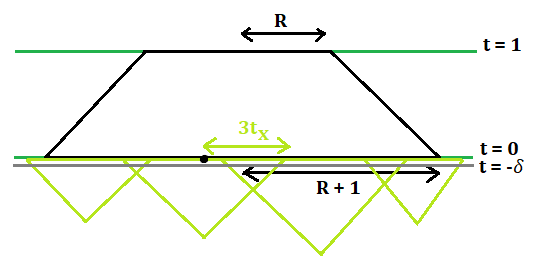
\includegraphics{graphics/blowup}
		\caption{The solution has small exterior energy and thus can be continued for some small time. If there is no energy concentration, we can cover the interior by a finite collection of light cones with small energy. Gluing together the local solutions, we can extend the whole solution uniformly in time. }
	\end{center}
\end{figure}	

By the exterior energy decay proved in Corollary \ref{cor:exterior}, it suffices to prove the result replacing the local energy in the light cone $\cE_{B_t (x_*)} [\phi[t]]$ with the energy in the larger cone $\cE_{B_{3t} (x_*)} [\phi[t]]$. Then, if energy does not concentrate, for each $x \in \R^d$ there exists $t_x \ll 1$ such that
	\[
		 \cE_{B_{3t_x} (x)} [\phi[t_x]] < \epsilon_*.
	\]	
To use the small data theory to rule out blow-up within the domain of dependence of, say, $B_{2t_x} (x)$ at time $t = t_x$, we need to localise in space, 

\begin{lemma}[Localisation of energy]\label{lem:local}
	Fix a cut-off $\chi \in C^\infty_c (\R^d)$ supported on the unit ball $|x| \leq 1$ and such that $\chi \equiv 1$ on the ball $|x| \leq \tfrac12$. Denote the rescalings $\chi_\lambda (x) := \chi(x/\lambda)$, then 
		\[
			||\nabla (\chi_\lambda \phi) ||_{L^2 (\R^d)} \lesssim_{d, ||\chi||_{L^\infty}, ||\nabla\chi||_{L^\infty}} ||\phi||_{L^{\frac{2d}{d - 2}} (|x|\leq \lambda)}  +  ||\nabla \phi||_{L^2 (|x| \leq \lambda)}.
		\]
\end{lemma}

\begin{proof}
	Computing the gradient of $\nabla (\chi_\lambda \phi)$ using the product and chain rules, and then applying the triangle inequality to the $L^2$-norm gives 
		\begin{align*}
			||\nabla (\chi_\lambda \phi) ||_{L^2 (\R^d)} 
				&\leq \lambda^{-1} ||\nabla \chi||_{L^\infty} || \phi||_{L^2 (|x| \leq \lambda)} + ||\chi ||_{L^\infty} || \nabla \phi||_{L^2 (|x| \leq \frac12 \lambda)} .
		\end{align*}
	To estimate the lower order term, we apply Holder's inequality,
		\begin{align*}
			 \lambda^{-1} || \phi||_{L^2 (|x| \leq \lambda)}
			 	&\leq  |B|\,  ||\phi||_{L^{\frac{2d}{d - 2}} (|x| \leq \lambda)},
		\end{align*}	
	where $|B|$ denotes the volume of the unit ball. This proves the result. 
\end{proof}

Applying the localisation lemma, we can apply a cut-off to obtain data $\phi^{\mathrm{reg}} [t_x]$ which has small energy and agrees with $\phi[t_x]$ on the ball $B_{2t_x} (x)$. By the small-data theory, the localised data admits a global solution $\phi^{\mathrm{reg}}$, while finite speed of propagation tells us that this solution agrees with $\phi$ in the domain of dependence of $B_{2t_x} (x)$ at time $t = t_x$. In particular, $\phi$ is regular in the ball $B_{t_x} (x)$ at time $t = 0$ and can be continued past this time. This completes the proof of Proposition \ref{prop:blowup}. That is, after translating in space, the solution blows up by concentrating energy inside a light cone towards the origin, 
	\[
		\limsup_{t \downarrow 0}\cE_{S_t} [\phi] \geq \epsilon_*. 
	\]
Following the proof of exterior energy decay, Corollary \ref{cor:exterior}, we can truncate the data at time $t_0 \ll 1$ so that the solution remains unchanged in the interior of the light cone $C_{[0, t_0]}$ and has small energy exterior to the light cone. We leave this as an exercise. 









